\section{Solução da calibração}
% TODO Gabriel e Elael: solução detalhada e final da calibração com simulações.

\subsection{Calibração da pá}

O formato original da pá do rotor é fixo para cara cada turbina, ou seja, uma
vez que definida em qual turbina será realizada a manutenção, é possível
fornecer \textit{a priori} qual tipo de pá será metalizada e suas
características. Essa característica possibilita descartar a necessidade de comparação e busca de
diversos modelos, reduzindo assim a complexidade computacional final do
algoritmo. Portanto, é possível armazenar uma representação de diferentes pás e
fornecer, como entrada do sistema, o modelo correto de acordo com o tipo de turbina que
está sendo inspecionada. O processo final consiste, então, no correto
posicionamento e alinhamento entre o modelo armazenado e a instância real do
objeto, ou mais especificamente a pá.

Os desenhos técnicos das pás, não fornecem informações suficientes
sobre o seu perfil hidráulico e, para fins práticos, os modelos serão adquiridos
a partir da inspeção \textit{in situ} de uma turbina em condições de conservação
que não apresente danos. Esse procedimento necessita ser realizado apenas uma
vez para cada modelo. Como especificado em \cite{EMMA DETAIL}, %TODO citar emma
% detail.
o sensor a ser adquirido pelo projeto é o Faro Focus X330. Esse dispositivo
consiste em um \texit{laser scanner} e aquisita a distância percorrida pelo
feixe $laser$ emitido pelo sensor até o obstáculo mais próximo. A partir de um
espelho rotativo e um motor acoplado em sua base, o Focus X330 é capaz de
aquisitar pontos em $360^o$ na horizontal e $300^o$ na vertical. O modelo de
cada pá será, então, uma nuvem de pontos representando tridimensionalmente todas
as caracterísiticas necessárias.

A partir da suposição que a pá se encontra dentro do campo de visão do sensor
$laser$, determinar a posição da pá consiste em posicionar a nuvem de pontos do
modelo de forma que ocorra uma sobreposição entre os pontos do modelo e da cena
e ambos conjuntos de pontos tenham as mesmas características, ou seja,
representem o mesmo objeto. A técnica a ser utilizada é denominada
\textit{correspondence grouping}. 


\subsubsection{\textit{Correspondence Grouping}}
 
O método proposto por \cite{Tombari2010a}, se baseia na identificação de
\textit{features} ou características tridimensionais locais para pontos de
interesse e identificar um conjunto de correspondências entre o modelo 3D e o a
cena analisada, no caso da aplicação do projeto EMMA as corresponências entre a
o modelo da pá e a turbina. Uma \textit{feature} descreve as caracteristicas da
vizinhança de um ponto, fornecendo assim informações locais para cada ponto. 

Para reduzir os cálculos necessários, é possível realizar uma amostragem na
nuvem de pontos e computar os descritores de cada caracteŕistica apenas para
pontos de interesse, tanto no modelo quanto na cena. Uma vez que ambos os
conjuntos de descritores foi calculado, deve-se então determinar as
correspondências entre os dois conjuntos. Pode-se utilizar, por exemplo, a
distância euclidiana entre os seus descritores correspondentes como medida
limite. Cada correspondência é uma evidência que o modelo se encontra na cena e
um acumulador é responsável por contabilizar os votos e um objeto é detectado
caso haja um número suficiente de votos. É importante ressaltar mesmo sendo
robusta a oclusões e ambientes com muita densidade de objetos, devido à presença de
ruído, e a particularidades de cada aplicação, como densidade e resolução das
nuvem de pontos forncecidas pelo sensor e pelo modelo, é possível a detecção de
falsos positivos, ou mesmo a incapacidade de se detectar corretamente o objeto
em questão. Para se tratar esse problema é necessário o correto ajuste de
diversos parâmetros e também a implementação de uma forma eficiente de avaliação
das hipóteses encontradas pelo algoritmo. 


\section{Simulação de nuvem de Pontos}

Devido a grande complexidade logística e a necessidade de disponibilidade de
acesso seco a uma turbina, é indispensável a possibilidade da sintetização de
dados consistentes e que representem de maneira eficaz as caracteristícas que
serão encontradas no cenário real de operação. 

\subsection{Dados genéricos}

Para um primeiro contato com o funcionamento do método \textit{Correspondence
Grouping} foram utilizados dados genéricos disponíveis na literatura
\footnotemark \footnotetext{http://kos.informatik.uni-osnabrueck.de/3Dscans/}
e um modelo da pá gerado pelo sensor Faro Focus X330 , durante a viagem de campo
à Usina Hidrelética de Jirau para o teste de viabilidade técnica desse sensor, foi
introduzido artificialmente na cena.

A figura \ref{fig::modelo_pa_faro} ilustra o modelo da pá em nuvem de pontos,
esse modelo é uma representação de $360^o$ da superfície da pá e foi aquisitado em
campo, sendo assim representa a real leitura final do sensor na aplicação do
algoritmo de calibração.

\begin{figure}[h!]
	\centering
	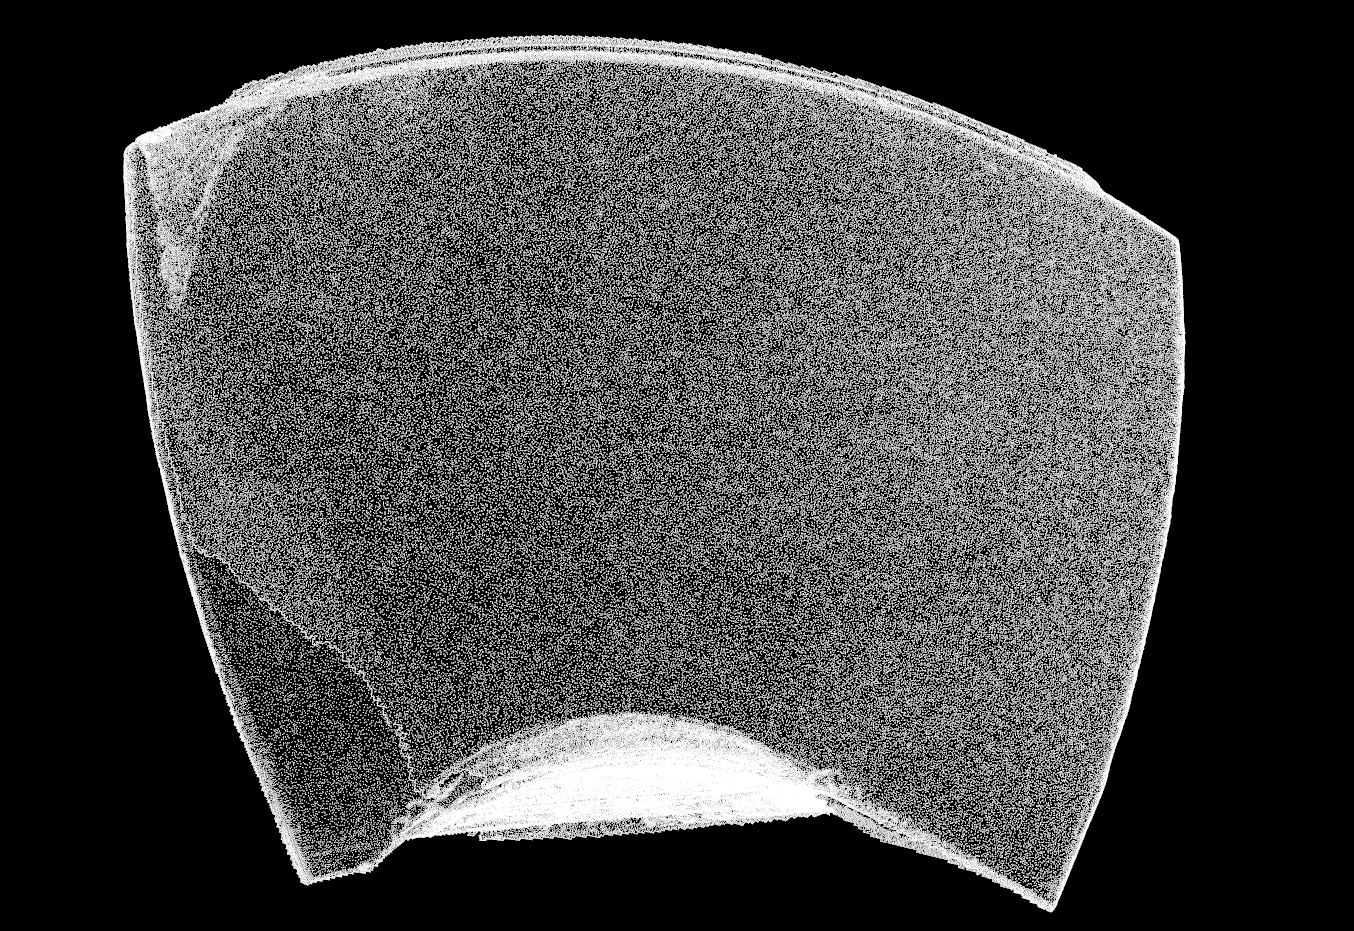
\includegraphics[width=0.9\columnwidth]{figs/calibracao/modelo_pa_faro}
	\caption{Nuvem de pontos da pá aquisitada pelo sensor Faro Focus X330.}
    \label{fig::modelo_pa_faro}
\end{figure}

A identificação da objeto na cena e a estimação da sua posição foi testada em
uma cena de um escritório, como pode ser visualizado na figura
\ref{fig::pa_cena_gen}. O modelo foi sobreposto em vermelho e não houve uma
discrepância visível entre a instância presente na cena e o modelo sobreposto. 
Mesmo com uma diferença de densidade de pontos presente em cada parte da nuvem
de pontos resultante (modelo é muito mais denso que a cena), foi possível
realizar a correta localização do modelo. O ajuste dos paramêtros de
subamostragem necessitaram de maior atenção nesse cenário. Vale ressaltar que o
algoritmo identificou corretamente uma cópia exata do modelo que foi introduzido
na cena, não há presença de ruídos ou oclusões no instância da pá presente na
cena.

\begin{figure}[h!]
	\centering
	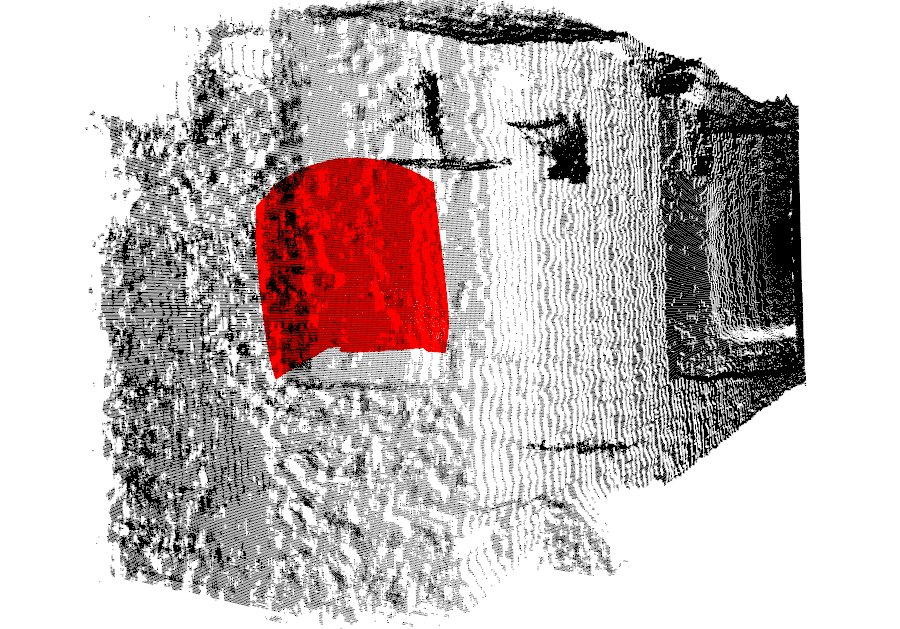
\includegraphics[width=0.9\columnwidth]{figs/calibracao/blade_office5}
	\caption{Exemplo de localização do modelo da pá em uma cena genérica.}
    \label{fig::pa_cena_gen}
\end{figure}

\subsection{Blensor}

A utilização de dados genéricos é útil para a implementação e testes do
algoritmo, entretanto não representa as condições reais que serão encontradas
durante o processo de metalização. A geometria da turbina, da pá, do manipulador
e também as oclusões geradas pelos elementos presentes necessitam ser simulados
para um perfeito ajuste do sistema. Para a simulação desses cenários, foi
utilizado a \textit{toolbox Blensor}\footnotemark
\footnotetext{http://www.blensor.org} baseada no \textit{software} de criação 3D
\textit{Blender}\footnotemark \footnotetext{http://www.blender.org}, o qual
permite a simulação da nuvem de pontos resultante de um sensor em um ambiente
tridimensional. Os objetos inseridos na cena são sólidos 3D, que podem ser
desenhados utilizando-se as ferramentas do próprio programa ou importados de
outros  em outros formatos suportados, como a partir do
Solidworks\textregistered por exemplo. A Figura \ref{fig::blensor_screen}
ilustra a utilização do software, assim como o modelo 3D da turbina importado. A
simulação leva em consideração a distância percorrida pelo pulso emitido, a
intensidade luminosa retornada ao sensor e o tempo decorrido durante o
sensoriamento \cite{Gschwandtner2011}, o que fornece uma melhor aproximação da
resposta do sensor para um ambiente simulado do que simplesmente a utilização de
uma técnica de \textit{raycast} pura.

\begin{figure}[h!]
	\centering
	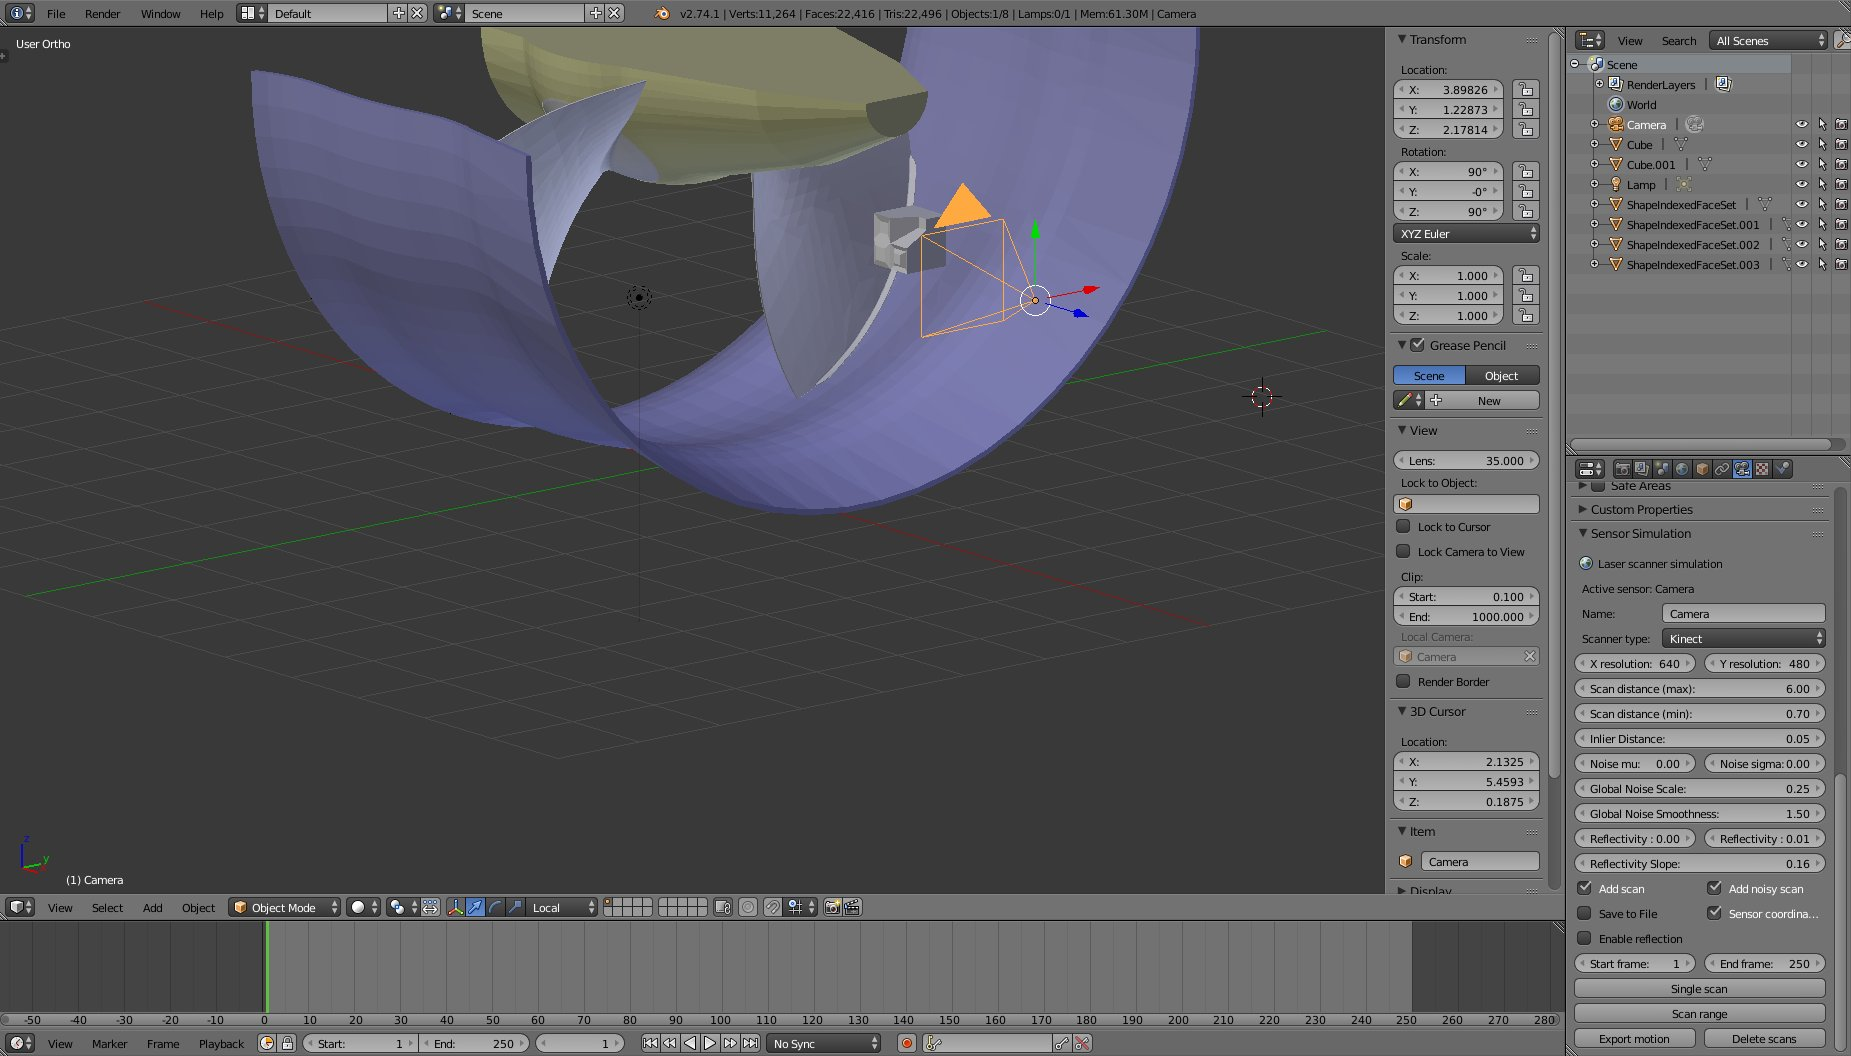
\includegraphics[width=0.9\columnwidth]{figs/calibracao/blensor_screen}
	\caption{Visualização do \textit{Blensor} com o modelo 3D da turbina
	importado.}
    \label{fig::blensor_screen}
\end{figure}

Dentro do ambiente de simulação, é possível a sintetização de dados provenientes
de diversos tipos de sensores laser, como um laserscanner 2D, o sensor
Velodyne e sensores do tipo Kinect. Os parâmetros de configuração
dos sensores também estão disponíveis para ajuste, assim como o nível de ruído. Sensores que não estão
nativamente disponíveis podem ser introduzidos. O sensor Faro Focus X330 não
pertence a lista de sensores previamente carregados pela ferramenta e teve que
ser implementado. As especificações técnicas utilizadas estão de acordo com as
fornecidas pelo fabricante, com exceção do ângulo de visão que foi reduzido para
diminuir o esforço computacional, sem perda de informação. A figura
\ref{fig::blensor_faro} ilustra a resposta simulada do sensor implementado
dentro do ambiente de simulação com a presença do modelo CAD da turbina.


 \begin{figure}[H]
	\centering
	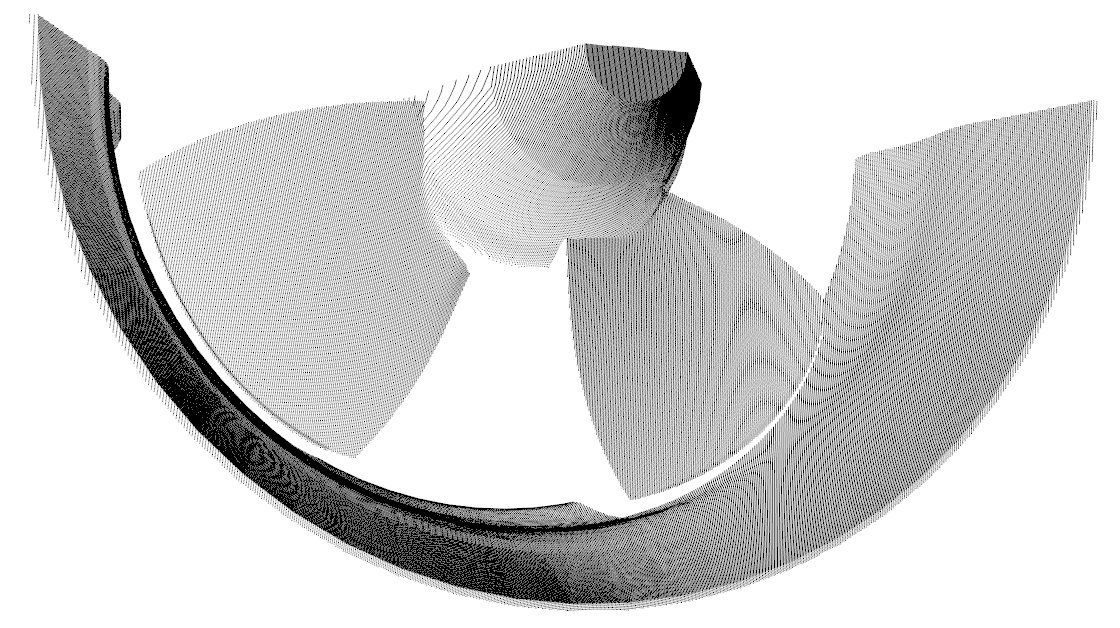
\includegraphics[width=0.9\columnwidth]{figs/calibracao/blensor_faro}
	\caption{Resposta simulada do sensor Faro Focus X330.}
    \label{fig::blensor_faro}
\end{figure}	


Caso seja disponibilizado uma descrição do perfil hidráulico da pá, é possível
também a geração de modelos sem a necessidade de uma inspeção prévia em uma
unidade geradora, na qual haja a presença de dados nas pás, para a aquisição de
dados sobre a turbina. A figura \ref{fig::modelo_pa} ilustra o ambiente de simulação e a
nuvem de pontos final para a criação de um modelo a partir de um arquivo
descritivo. 


\begin{figure}[h!]
	\centering
	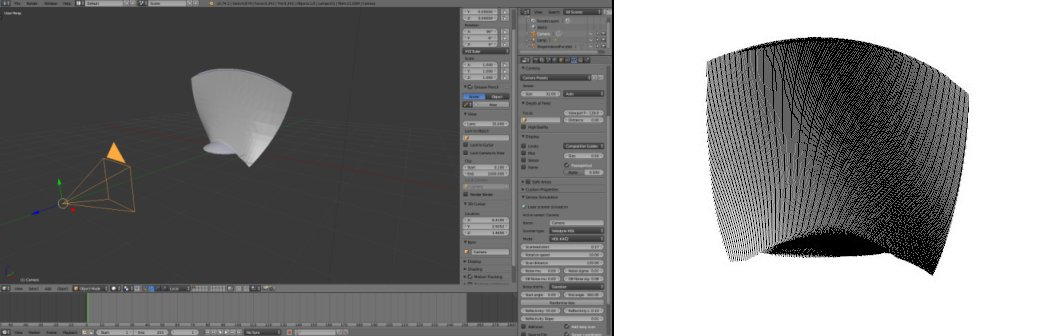
\includegraphics[width=0.9\columnwidth]{figs/calibracao/blensor_pa_sim}
	\caption{Criação de um sensor a partir de um arquivo descritivo da pá.}
    \label{fig::modelo_pa}
\end{figure}

Para representar corretamente as oclusões geradas pelo própria estrutura do
rotor e das pás, é necessário que as cenas sintetizadas a partir da ferramenta
tenham o sensor virtual posicionado em posições que representem os locais no
qual é possível a fixação real do equipamento dentro da UG. As oclusões geradas
pelo sistema de metalização também devem ser previstas e simuladas para um
perfeito ajuste do algoritmo, uma vez que o conjunto do robô e trilhos deve
estar previamente posicionado para que a calibração entre a pá e o efetuador do
manipulador seja realizada. Para isso, o modelo do manipulador MH12 foi
importado para dentro do ambiente de simulação, como ilustrado na figura
\ref{fig::model_mh12} e, em seguida, posicionado entre o sensor e a pá, para
servir de obstáculos para parte dos feixe laser que atingiriam a pá.


\begin{figure}[H]
	\centering
	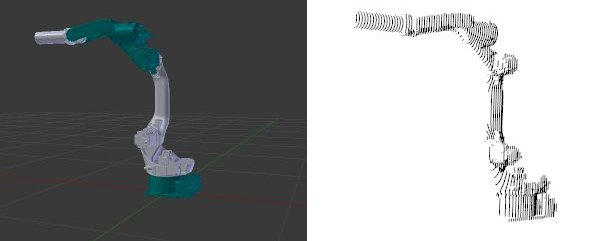
\includegraphics[width=0.9\columnwidth]{figs/calibracao/mh12_model}
	\caption{Visualização do \textit{Blensor} com o modelo 3D da turbina
	importado.}
    \label{fig::model_mh12}
\end{figure}

A Figura \ref{fig::sim_mh12}
ilustra a pá sendo corretamente identificada com a presença do manipulador entre
o sensor e a pá criando uma região de sombra. É possível observar o modelo que
está sendo comparado à cena na parte direita da figura e as linhas verdes
representam as correspondências encontradas entre os descritores do modelo da pá
e os encontrados na cena.

\begin{figure}[H]
	\centering
	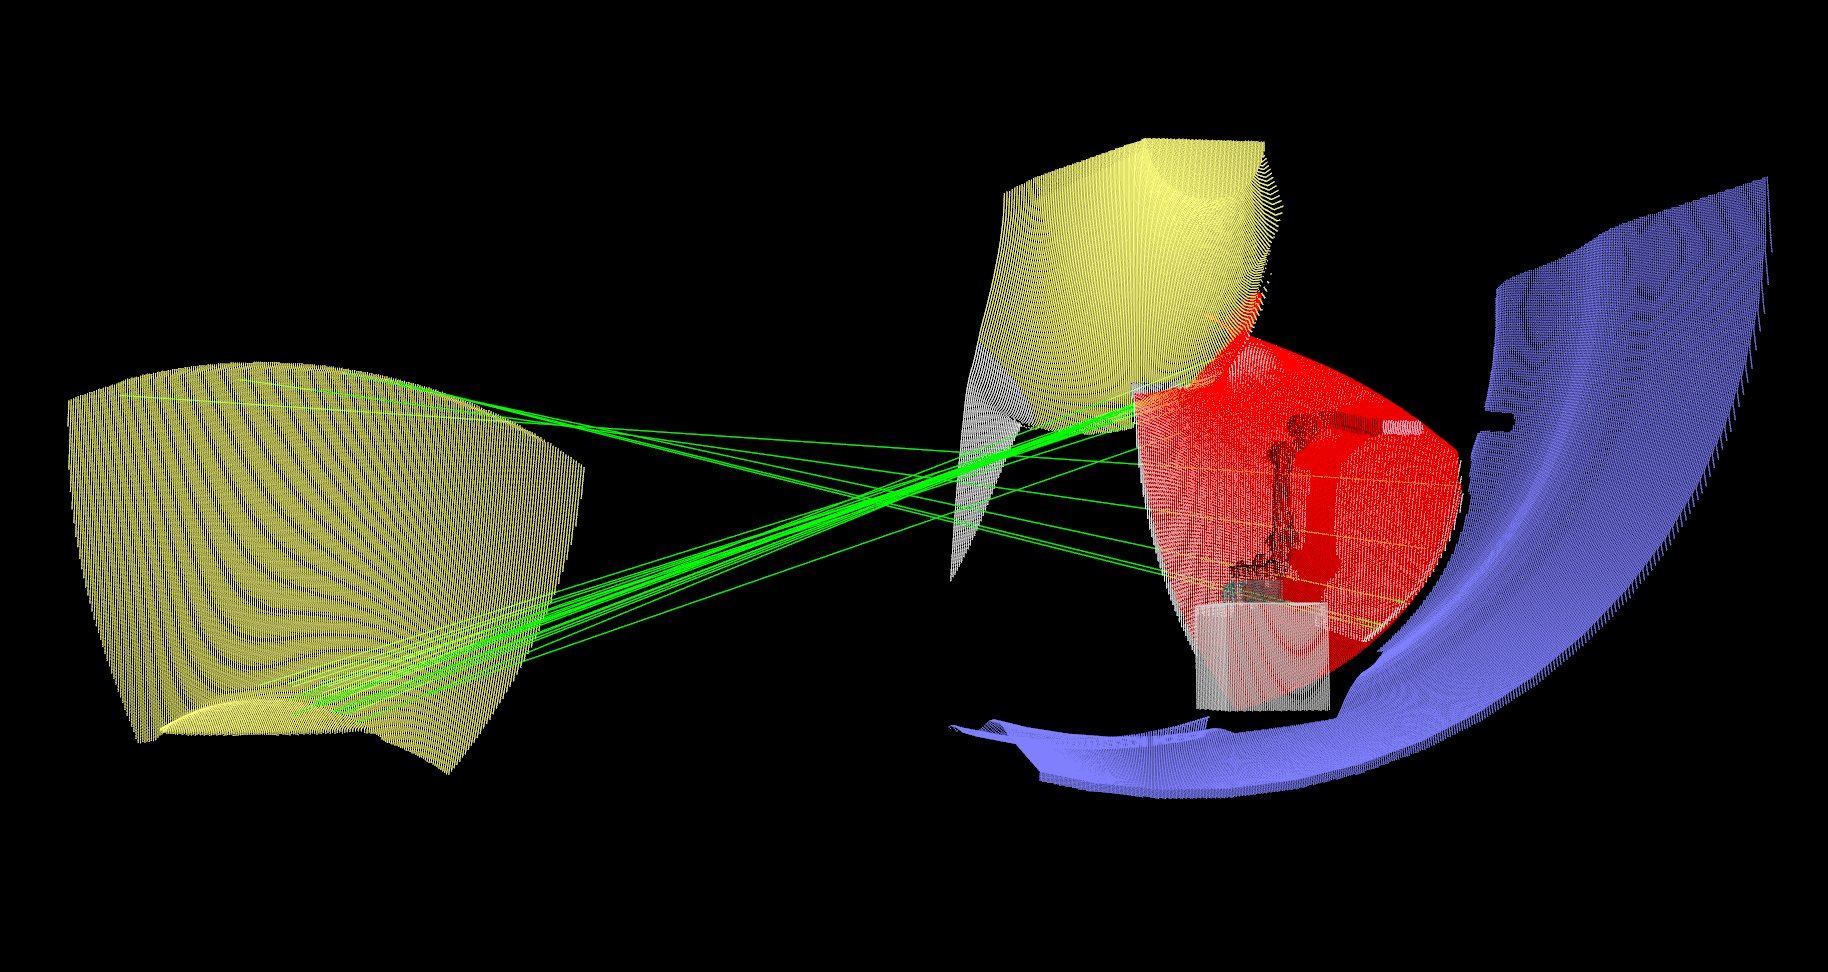
\includegraphics[width=0.9\columnwidth]{figs/calibracao/sim_mh12_sp}
	\caption{Resposta simulada do sensor Faro Focus X330.}
    \label{fig::sim_mh12}
\end{figure}	
